\subsection{Kiến trúc hệ thống}

Kiến trúc của hệ thống hoạt động theo như Hình 4.7

\begin{figure}[H]
    \centering  
    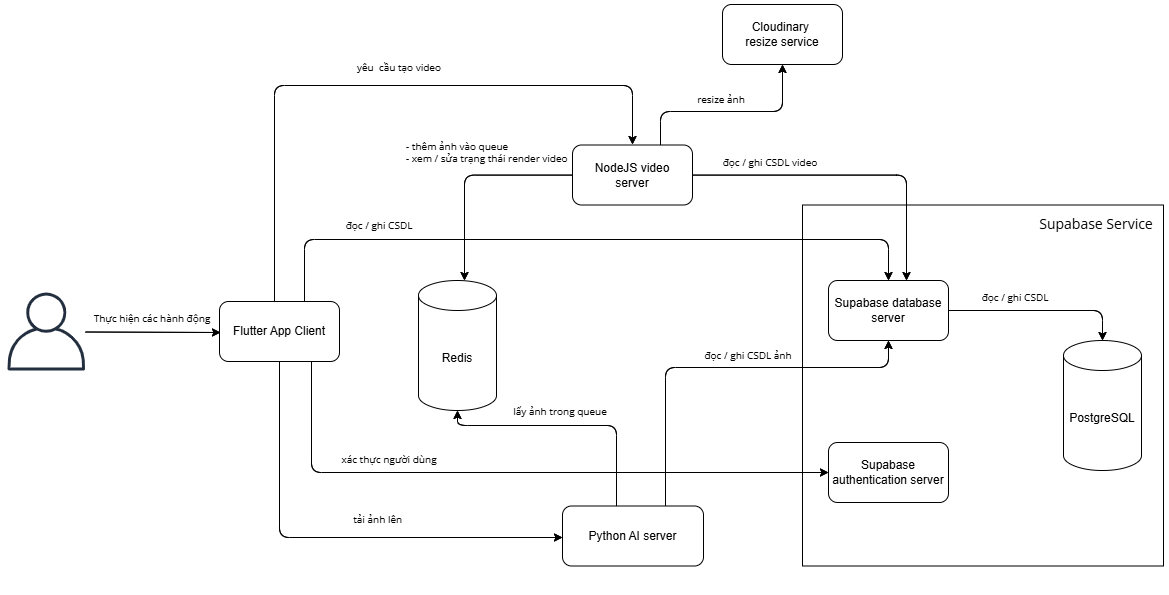
\includegraphics[width=1.1\textwidth]{figures/c4/4_1/architechture.png}
    \caption{Biểu đồ kiến trúc hệ thống.}
    \label{fig:architecture_diagram}
\end{figure}

\textbf{Flutter App Client:} cung cấp giao diện giúp người dùng có thể tương tác với hệ thống. Client sẽ giao tiếp với các dịch vụ thông qua API để thực hiện các chức năng như xác thực người dùng, tương tác với database, render video, đánh nhãn ảnh và phân loại khuôn mặt trong ảnh.

\textbf{Redis:} đóng vai trò là một bộ nhớ cache lưu thông tin tạm thời cho các dịch vụ trong hệ thống. Cụ thể như sau: 
\begin{itemize}
    \item[-] Lưu thông tin render video: NodeJS video server sẽ lưu trữ trạng thái của video trong Redis để có thể truy xuất nhanh chóng và đồng thời hạn chế người dùng chỉ được phép render video một lần trong một khoảng thời gian nhất định.
    \item[-] Công cụ giao tiếp giữa các dịch vụ: hệ thống sử dụng Redis stream như 1 hàng đợi để đánh dấu những ảnh cần được gán nhãn. Khi NodeJS server phát hiện có ảnh nào trong request tạo video chưa được gán nhãn, server sẽ gửi thông tin ảnh đó vào Redis stream. Python AI server sẽ lắng nghe Redis stream và khi có thông tin ảnh mới, server sẽ lấy ảnh từ kho dữ liệu của Supabase Service, thực hiện gán nhãn cho ảnh và lưu lại kết quả vào kho dữ liệu của Supabase 
\end{itemize}

\textbf{NodeJS video server:} cung cấp dịch vụ render video cho người dùng. Server này sẽ nhận request tạo video từ client, sau đó resize ảnh bằng Cloudinary resize service, tạo video và lưu video vào kho dữ liệu của Supabase Serivce. 

\textbf{Python AI server:} cung cấp dịch vụ gán nhãn ảnh cho người dung. Ngoài ra server cũng thực hiện việc nhận diện khuôn mặt trong ảnh và nhóm những khuôn mặt tương tự nhau để người dùng có thể dễ dàng tìm kiếm và phân loại ảnh. 

\textbf{Supabase Service}: được sử dụng cho các chức năng như lưu trữ ảnh, video, thông tin người dùng và lắng nghe thời gian thực về sự thay đổi của dữ liệu. Bao gồm các dịch vụ như sau:
\begin{itemize}
    \item[-] Supabase database server: lưu trữ các bảng dữ liệu như users, videos, images, faces, v.v. và các dữ liệu tệp tin khác như ảnh, video.
    \item[-] Supabase authentication server: thực hiện xác thực và ủy quyền người dùng. Hệ thống sử dụng JWT token để xác thực người dùng và phân quyền truy cập cho các dịch vụ trong hệ thống.
    \item[-] PostgreSQL: là hệ quản trị cơ sở dữ liệu được Supabase sử dụng.  
\end{itemize}

\textbf{Cloudinary resize service}: cung cấp dịch vụ resize ảnh cho hệ thống. Hệ thống sử dụng Cloudinary để resize ảnh trước khi tạo video, nhằm tăng tốc độ tạo và giảm dung lượng tạo video.
